%%%%%%%%%%%%%%%%%%%%%%%%%%%%%%%%%%%%%%%%%%%%%%%%%%%%%%%%%%%%%%%%%%%%%%%%%%%%%%%%%%%%%%%%%%%%%%%%%%%%%%
%
%   Filename    : chapter_3.tex 
%
%   Description : This file will contain your Research Methodology.
%                 
%%%%%%%%%%%%%%%%%%%%%%%%%%%%%%%%%%%%%%%%%%%%%%%%%%%%%%%%%%%%%%%%%%%%%%%%%%%%%%%%%%%%%%%%%%%%%%%%%%%%%%

\chapter{Theoretical Framework}
This chapter contains theories and concepts that are related to the research.

\section{Symphonies}
\subsection{Basic Structure of a Symphony}
The Classical and Romantic symphony is mainly written in four movements, namely the fast tempo or sonata allegro form, the slow tempo, the medium/fast tempo or minuet, and the fast tempo again. The sonata form makes up the main form of Classical and Romantic symphonies. It is composed of two contrasting themes, the aggressive and the passive and is further divided into several sections, namely the introduction, exposition, development, recapitulation, and coda. The introduction section is purely optional and is slow and solemn in nature. The exposition section is where the themes of the symphony are “exposed” or presented for the first time and will consequently be repeated all throughout. The development section is where the themes are altered and manipulated. The recapitulation section is where the themes return to their original forms from before they were altered. The code section finally represents the end of the movement and this is where the original tone from the exposition section is repeated or recapped to form the ending for the movement (Heikkinen, 2017 \& BBC, 2014).

\subsection{Music Features}

A feature is a characteristic used to distinguish one entity from another and in a sense defines its uniqueness. Music features, therefore, are what makes music similar to or different from one another. By comparing the values  for each music feature and by examining if a feature is present at all or not, comparison of music by mathematical means is very possible (Huron, 2001).

Today, music information retrieval (MIR) has become an important area of research especially because of the ever expanding database for music through the years. The features extracted from music can be used in many areas of MIR research. It can be said that when two songs share closer values for each music feature, then they are more similar than with others (Corrêa \& Rodrigues, 2016).

\subsubsection{MFCC}

MFCC, also known as Mel-Frequency Cepstral Coefficients, is the most commonly used feature in speech analysis and since speech analysis and music research are closely interrelated as pointed out by Loughran, Walker, O'Neill, \& O'Farrell (2008), then MFCC will likely be the most commonly used feature in music feature extraction.

According to Lutter (2014), MFCC is based mainly from experiments on human misconceptions of words such as when a person misunderstands what another person says. This feature extraction method was first developed by Bridle and Brown in 1974 and was further developed by Mermelstein (1976).  The MFCC feature extraction method involves mimicking some parts of the human speech production and speech perception. This feature extraction involves five steps, namely the fourier transform, the mel-frequency spectrum, the logarithm, cepstral coefficients, and the derivatives. The first step, fourier transform makes use of the formula $C_r,_k=| \frac{1}{N}\sum_{j=0}^{N-1} fj exp [-i 2 \pi \frac{jk}{N}]|$, where $k=0,1,...,(\frac{N}{2})-1$ and N is the number of samples within a speech or time frame.

The mel-frequency spectrum closely mimics the sensation of the human ear's auditory system and the process involves filtering the spectrum with different band-pass filters, devices that pass frequencies within a certain range and reject all others, and the power for each band-pass filter is computed accordingly (Agarwal, 2017). The computation makes use of the formula $C_T,_j=\sum_{k=0}^{\frac{N}{2}-1} d_j,_k C_T,_k $, where $j=0,1,...,N_d$ and d is the amplitude of the band-pass filters at index j and frequency k, to produce the corresponding filter bank for the spectrum.

The third step, logarithm involves mimicking the perception of loudness by the human ear and is represented by the formula $C_T,_j= log(C_T,_j)$  where $ j=0,1,...,N_d$.

In cepstral coefficients, the main goal here is to remove the speaker or the music dependent characteristics. The computation of cepstral coefficients results in the inverse of the fourier transform of the estimated spectrum of the signal and is represented by the formula $C_T,_j=\sum_{j=1}^{N_d} C_T,_j cos[\frac{k(2j-1)\pi}2N_d]$ where $k=0,1,...,N_m,_c<N_d$ and $N_m,_c$ is the chosen cepstral coefficient for further processing.

Lastly, the derivative represents the dynamic nature of speech or the music.

\section{Preprocessing}
\subsection{Data Collection}

In gathering data, a careful lookup for patent or copyright issues must strictly be observed. Symphonies are musical pieces that were generally composed a long time ago and as such copyright on the actual symphonies are nonexistent. The only copyright issues to be possibly encountered here would be the source of the recreated symphony. For example, when the symphony is uploaded by a certain person in Youtube then the standard youtube license or the creative commons would apply (Brown,  2017).

\subsection{Preparation of Dataset}

In Azcarraga \& Flores (2016)'s research regarding visualization and comparison of symphonies through SOM, the preparation of dataset was done by first cutting the symphony into multiple 1 second music segments with an overlapping interval of 0.5 second to provide a smoother transition of the segments when represented later visually in addition to taking consideration of sections or notes that have been abruptly cut during the splitting process. In this way, after the feature is extracted and trained in the SOM, the multiple music segments will make up different musical trajectories which makes up the map visualization.

\subsection{Feature Extraction}

Feature extraction is the means of extracting relevant and effective data to train machine learning algorithms. Not all features, however, may be useful and others may be irrelevant individually but can be useful when combined with other features. The input data or “raw” data often need to be converted into a set of useful features through preprocessing transformations such as, standardization, normalization, signal enhancement, nonlinear expansion, et al. The resulting data may also be pruned of excess features in order to achieve improved algorithm speed and or predictive accuracy (Guyon \& Elisseeff, 2006).


Feature extraction for music can be done using jAudio, a Java project/program developed by McEnnis, McKay, Fujinaga, \& Depalle (2005). JAudio is a feature extraction system that provides a user friendly GUI and a command line interface to suit user needs for selecting their desired features to be extracted for the audio. The system accepts audio files as input and outputs XML or ARFF files. This output file contains the values for each feature of the audio file selected by the user.

\subsection{Feature Selection}

Gupta (2017) defines decision tree as a binary tree that branches down from the root. The term tree-walking is used to continuously make decisions on every level of the tree starting from the root node until the leaf nodes are reached or a satisfactory answer is found. In this way, it can be derived that the nodes found at the top of the tree are more important than its child nodes and all others beneath them. Decision trees are useful for inferring what features of a dataset can greatly or weakly influence its outcome (Mitchell, 1997).

Feature selection is the automatic selection of attributes in the dataset that are most relevant to a specific predictive model. It seeks to identify the out of the ordinary features among all the others and it helps in reducing the number of data attributes being used while still retaining a good or accurate predictive model. Aside from reducing the number of features or data attributes, it can also help in removing unwanted attributes that may decrease the accuracy of the predictive model (Brownlee, J., 2014).

Grabczewski \& Jankowski (2005) explains that decision tree algorithms are best used for feature selection because of the inherent characteristic of decision trees that allows them to separate the different features and showcase the more important features since it will appear at the root of the decision tree.
	
Some simple but successfully tested algorithms for feature selection would include Pearson's correlation coefficient and Fisher-like criterion. Pearson's correlation coefficient or Pearson's R is widely used in the computation of statistics and this involves detecting linear correlation, which is the representation of how close the data points are in making a straight line in a graph, just as shown in Figure 3.1.

\begin{figure}[h]
\caption{Pearson Correlation Graph}
\centering
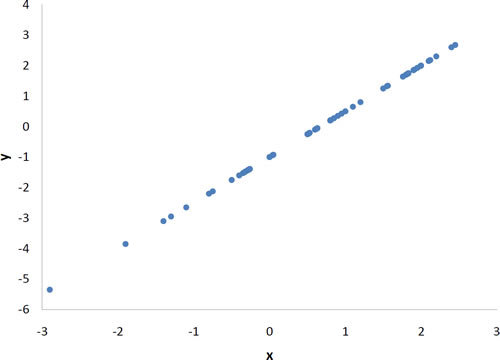
\includegraphics{pearson}
\end{figure}

PCA is another statistical procedure that transforms a set of data points using orthogonal transformation, which scales the set of points by a certain value, into a set of linearly uncorrelated values called principal components. Principal components are ordered such that the variance from the original variable decreases. It will always turn out that the first principal component will have the largest variance that was present in the original variable.

In machine learning, PCA is used to reduce the dimensionality of a set of data points. In implementing PCA on a 2D data set, the mean and the covariance of the data set would first have to be computed first. Mean is computed using $m = \frac{1}{P}\sum_{\mu=1}^{p} x^\mu$ and Covariance is measured using $S = \frac{1}{P-1}\sum_{\mu=1}^{P} (x^\mu-m)(x^\mu-m)^T$ (Storkey, 2017).

The eigenvalue and the eigenvector would also have to be computed. Eigenvector is computed using the formula $det(\lambda I - A ) = 0$, where $\lambda$ is the eigenvalue, I is the identity matrix of A, det is the determinant of the matrix, and A is the covariance matrix from the previous step. Eigenvalue is computed using the formula $( \lambda I - A )v = 0$.

For each data point $x^n$, the lower dimensional representation is $y^\mu = E^T(x^\mu - m)$ and the approximate reconstruction of the original data point $x^n$ is $x^\mu = m+Ey^\mu$. The total squared error over all the training data made is given by $(P-1)\sum_{j=M+1}^{N} \lambda j$ where $\lambda j , j = M + 1 . . . N$ are the eigenvalues discarded in the projection.

The last step is to choose the components and to form the feature vector. The number of eigenvectors and eigenvalues is equal to the number of data in the dataset. The eigenvector corresponding to the highest eigenvalue is the principal component of the dataset. To form the feature vector, the top k eigenvectors with top eigenvalues will be  used. To compute for the principal component, the transposed version of the feature vector is left-multiplied with the transposed version of the scaled version of the original dataset.

Fisher-like criterion makes use of the formula $\frac{m_0-m_1}{s_0-s_1}$, wherein m is the mean value of the feature for the$i$-th element and $s$ is the corresponding standard deviation. This algorithm can only be used, however, when dealing with binary classifications.

Feature selection, in general however, can be classified into three categories, namely the filter methods, wrapper methods, and the embedded methods. Filter method involves labelling each feature with a statistical measure and by comparing these measures, the more important features can be selected. Wrapper method involves grouping different combinations of features together to see which combinations work best. Embedded methods involve learning which features best contribute to the accuracy of the model while the model is simultaneously being created. Some more examples of feature selection algorithms would include best-first search, hill-climbing algorithm, and the usage of heuristics. Best-first search and hill-climb fall under the wrapper methods wherein different combinations are used until the top n features are found. Heuristics falls under the filter method wherein a heuristic score is given to each feature using a statistical measure such as Euclidean distance for example, and the features with the high scores will be the ones selected.

\section{Machine Learning}

Machine learning as defined by Ng (2017) is the science behind computers acting on a certain stimulus without being explicitly programmed to do so. Some examples of impact led by machine learning would be self-driving cars and web search suggestions from Google. Machine learning is also widely used in many different fields of research such as in artificial intelligence, data mining, natural language processing, image recognition, and expert systems (McCria, 2014). In machine learning, the concept of training the system to perform a unique task given a certain amount of data received has two main underlying categories, unsupervised learning and supervised learning.

\subsection{Supervised Learning}

Supervised learning, as defined by Brownlee (2016), is a type of machine learning wherein an input variable and an output variable is defined and an algorithm is used to map the input to the output variable. The goal of this type of learning is to map the input variables to their respective output variables by approximation so that when a new input variable is presented, an output can be predicted by the system. The main difference of supervised learning over unsupervised is that there is no third party that supervises and corrects the training of data in unsupervised but in supervised, intervention of the supervisor is necessary in order to achieve an acceptable level of performance by the system. Supervised learning can be further divided into two groups, namely regression and classification. Regression is used when the output is a real value, for example, weight, height, or age. Classification is used when the output is a category or group, for example, colors, sizes.

\subsection{Unsupervised Learning}

Brownlee (2016) defines unsupervised learning as having no corresponding output variable. Unsupervised learning is analysing the structure and distribution of the data in order for system to learn. Unsupervised learning can be further classified into two groups of algorithms, namely the clustering and the association. Clustering is used for discovering the groupings of data through clusters and association is used for discovering rules that describe the provided data.

\subsubsection{SOM}
Teuvo Kohonen (1995) defines SOM as a data visualization technique developed by Professor which reduces the dimension of data through the use of self-organizing neural networks. As SOM reduces the dimension of data, it also groups similar data items together; therefore, it not only reduces the dimension of data but also groups similar ones together. Figure 3.2 shows a basic example of a SOM. Note in this example that the data represented by colors are grouped according to their similarity (eg. yellow is near orange, dark teal is between blue and green).

\begin{figure}[h]
\caption{SOM Sample}
\centering
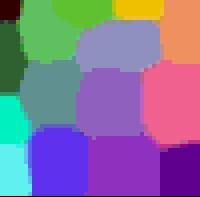
\includegraphics{som}
\end{figure}

Rumelhart \& Zipser (1985) defines a class under supervised learning called competitive learning. Here, neurons compete among themselves in a winner-takes-it-all scenario wherein only one neuron wins and is activated at any one time. Implementation of this competition is done through the use of lateral inhibition connections, which are structures of a network in which neurons inhibit their neighbors. When neurons are forced to organize themselves through this scenario, then the result would be a map that is self-organized, thus a SOM.

\subsubsection{K-Means Clustering Algorithm}

K-means clustering algorithm is a type of unsupervised learning algorithm wherein a set of unlabeled data will be grouped together and these groups are defined as the k variable. The algorithm will assign the different data points to their respective k-groups based on the selected features. Data points will then end up being clustered based on their feature similarities. The algorithm has two main iterative steps, , the data assignment step and the centroid update step, that repeats until either data points change clusters, the sum of the distances is minimized, or some maximum number of iterations is reached. Before starting with these two steps, the centroid for each k-cluster is computed first. In data assignment, each data point is placed in their nearest centroid value computed with squared Euclidean distance. In centroid update, the centroid is recomputed by taking the mean of all the data assigned to the cluster of the centroid (Hartigan \& Wong, 1979).

\subsubsection{t-SNE}

Maaten \& Hiton (2008) introduces t-SNE as a variant of the Stochastic Neighbor Embedding (SNE) which seeks to visualize high dimensional data by plotting these data points in a two or three dimensional map. Since t-SNE is a variant of SNE, SNE would have to be discussed first before transitioning to t-SNE. SNE starts by transforming the Euclidean distances of the high-dimensional data points into conditional probabilities that represent similarities. For example with $p_{j|i}$, this would represent the similarity from $X_j$ to $X_i$, that $X_i$ would pick $X_j$ as its neighbor if neighbors were picked in proportion to their probability density under a Gaussian centered at $X_i$. The conditional probability of $p_{j|i}$ is given with $p_{j|i} = \frac{exp(-||x_i-x_j||^2 /2 \delta_i^2}{\sum_{k \neq i} exp(-||x_i - x_k||^2 / 2 \delta_i^2}$ where $\delta i$ is the variance of the Gaussian that is centered in $X_i$. $p_{i|i}$ is set to 0 since only pairwise similarities will be considered. For the low dimensional counterpart of $X_i$ and $X_j$, the probability is computed by $q_{j|i} = \frac{exp(-||y_i - y_j||^2}{\sum_{k \neq i} exp(-||y_i - y_k||^2)}$.

As with its high dimensional counterpart, $q_{i|i}$ is set to 0. In order for SNE to find a low dimensional data representation that represents the mismatch between $p_{j|i}$ and $q_{j|i}$, a cost function is used, $C = \sum_{i} KL(P_i||Q_i) = \sum_{i}\sum_{j} p_{j|i} log \frac{p_{j|i}}{q_{j|i}}$,where KL is the Kullback-Leibler divergences, $P_i$ is the conditional probability distribution over all other data points given data point $X_i$, and $Q_i$ is the conditional probability distribution over all other data points given data point $Yi$.

With the variance $\delta i$  of the Gaussian that is centered over each high-dimensional data point $X_i$, it is important to note that the density of all data points in a data set are not uniform and it is more appropriate to use a smaller $\delta i$ value in denser regions than in sparser regions. Any value of $\delta i$ influences a probability distribution $P_i$ over all other data points. This probability distribution has an entropy value which increases as $\delta i$ increases. SNE seeks for a value of $\delta i$ that has a $P_i$ with fixed perplexity specified by the user using binary search. The perplexity is computed by $Perp(P_i) = 2^{H(P_i)}$ where the $H(Pi)$ or the Shannon entropy of $P_i$ is further computed using $H(P_i) = -\sum_{j} p_{j|i} log_2 p_{j|i}$. The smooth measure of the effective number of neighbors can also be identified as the perplexity and the typical values for this would range from 5 to 50. The cost function shown earlier can also be minimized into $\frac{\delta C}{\delta y_i} = 2\sum_{j} (p_{j|i} - q_{j|i} + p_{i|j} - q_{i|j})(y_i - y_j)$.

The gradient can be thought of as a spring force from a map point $y_i$ to any $y_j$ along the map. As the force is computed with $y_i-y_j$, the resulting force can either make the points repel or attract each other depending if the distance between the two is too small or too large. To speed up the optimization and to avoid poor local minima, a gradient update with a momentum term is done using $y^{(t)} = y^{(t-1)} + \eta \frac{\delta C}{\delta y} + \alpha (t) (y^{(t-1)}-y^{(t-2)})$ where $y^t$ indicates the solution at iteration t, $\eta$ indicates the learning rate, and $\alpha (t)$ represents the momentum at iteration t.

In t-SNE, certain issues such as the crowding problem, which is when too many data points get crowded in a map with a small number of dimension such as with 2D or 3D, are tackled by using a symmetrized version of the SNE cost function with more simple gradients and to use Student t-distribution instead of the Gaussian distribution when computing similarity between two low-dimensional points. The alternative cost function for a symmetrized SNE is $C=KL(P||Q) = \sum_{i}\sum_{j} p_{ij}log\frac {p_{ij}}{q_{ij}}$ where $p_{i|i}$ and $q_{i|i}$ are set to 0 just as in SNE and $p_{ij}$= $p_{ji}$ as $q_{ij}$= $q_{ji}$ since they constitute the symmetric property. $p_{ij}$ is computed using $p_{ij} = \frac{exp(-||x_i - x_j||^2 / 2 \delta ^2 )}{\sum_{k \neq 1}exp(-||x_k - x_l||^2 / 2 \delta ^2 )}$ and $q_{ij}$ using $q_{ij} = \frac{exp(-||y_i - y_j||^2)}{\sum_{k \neq 1}exp(-||y_k - y_l||^2)}$. In order to avoid having $p_{ij}$ with extremely small values which results from outliers, $p_{ij}$ is first set by $p_{ij} = \frac{p_{j|i} + p_{i|j}}{2n}$ so that $\sum_j p_{ij} > \frac{1}{2n}$ for all data points $x_i$. The gradient of symmetric SNE is computed using $\frac{\delta C}{\delta y_i} = 4 \sum_j (p_{ij} - q_{ij})(y_i - y_j)$.

In t-SNE, just as discussed above, Student t-distribution with one degree of freedom will take the place of Gaussian distribution as the heavy-tailed distribution in the low-dimensional map. $q_{ij}$ will now be computed using $q_{ij} = \frac{(1+||y_i - y_j||^2)^{-1}}{\sum_{k \neq 1} (1+||y_k - y_l||^2)^{-1}} $. A student t-distribution with one degree of freedom is used because it has the property $(1+||y_i - y_j||^2)^{-1}$  wherein it  approaches an inverse law for large pairwise distances in the low dimensional map. The resulting map representation of joint probabilities will make the map points invariant to changes in the scale of the map. Large clusters of points that are far apart will also interact just the same way as how an individual point would.

The gradient of the Kullback-Leibler divergence between P and the Student t-based joint probability distribution Q can be computed using $\frac{\delta C}{\delta y_i} = 4\sum_j (p_{ij} - q_{ij})(y_i - y_j)(1+||y_i - y_j||^2)^{-1}$. The resulting gradient from t-SNE will strongly repel dissimilar data points resulting in a visual image that clearly separates each data class as can be clearly seen in the t-SNE results in Appendix E as compared with the results from the other dimensionality reduction techniques used.

In their experiment set-up, they used a total of three data sets as was discussed back in Chapter 2 which includes the MNIST data set, the Olivetti faces data set, and the COIL-20 data set. They first used PCA to reduce the dimensionality of the data to 30 so that the computation of pairwise distances between data points would be faster and at the same time also suppresses the noise without severely distorting the distances between the data points. They then applied different dimensionality reduction techniques which includes Sammon mapping, Isomap, and LLE to compare the resulting visualization later on with the result of t-SNE. The results of each data set for each technique on the MNIST data set can be viewed in Appendix E. The coloring scheme in the visual images represent each class of data. The cost function parameter they used for their experiment was Perp = 40 for t-SNE, none for Sammon mapping, and k = 12 for Sammon mapping and Isomap.

Their results show that t-SNE overall had better visualization because the data classes are more distinct or separated than compared with the results from the other methods.  In general, t-SNE outperformed all the other dimensionality reduction techniques used in their research; however, the authors point out that t-SNE has three general weakness to consider. The first one is that it is unclear how t-SNE will perform on the more general task of dimensional reduction. In other words, if dimensionality is increased to more than 3, it is unclear whether t-SNE will still produce optimal visualization results. One way of addressing this problem is to optimize the Student t-distribution to have more than one degree of freedom. The second weakness is the curse of intrinsic dimensionality since t-SNE only reduces the dimensionality of data based on the local property of the data. Data sets that have high intrinsic dimensionality and an underlying manifold that is highly varying causes the local linearity of assumption on the manifold that t-SNE implicitly makes be violated; therefore, applying t-SNE to data sets with high intrinsic dimensionality can produce unreliable results. One way to address this problem is to perform t-SNE on a data representation obtained from a model that represents the highly varying data manifold efficiently in a number of non-linear layers. The last weakness is the non-convexity of the t-SNE cost function. Since the cost function of t-SNE is non-convex, several optimization parameters would first have to be chosen. The constructed solutions would then vary depending on the optimization parameter used each time from an initial random configuration of map data point. They explicitly point out however that the same choice of parameters can be used for different visualization tasks and the result would still be of similar

\section{Visualization}
\subsection{Single Image}

Just as done in Azcarraga \& Flores (2016)'s research work and in Maaten \& Hiton (2008)'s t-SNE, visualization for the result of the SOM and t-SNE is projected in a single image. With SOM, the BMU or best matching unit, which will be explained further in section 3.5.1, represents the music trajectory of a certain 1 second music segment from the symphony. This sequence of BMUs make up the visual image representation of a certain symphony. A color coding scheme was also used to denote the time sequence of a certain music trajectory in the image, blue representing the start and going to red as the music progresses as shown in Figure 3.3. For t-SNE, sample visual images can be seen in Appendix E.

\begin{figure}[h]
\caption{SOM Image from SOMphony}
\centering
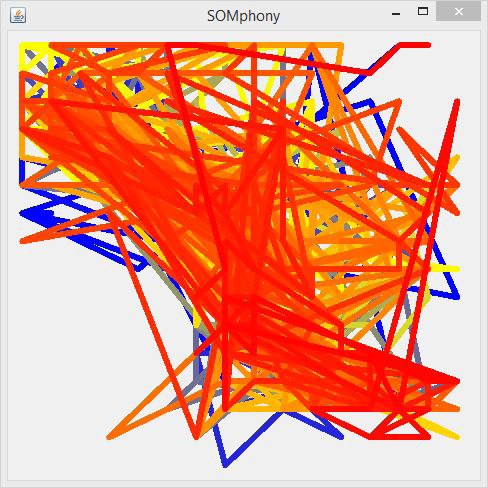
\includegraphics[width=0.5\textwidth]{somphony_sample}
\end{figure}

\subsection{Video}
Aside from representing the result of the SOM in a single image, it can also be represented in a video or multiple images. Video can be produced for the results of this research by collating  each 1 second segment result in order to show the progression of the musical trajectory grow from the start of the symphony to the end. This allows clearer visualization of the data to have more accurate analysis. Using this kind of visualization also greatly helps the survey user in the outcome of this research.

\subsection{3D Models}

In Azcarraga, Caronongan,  Setiono, \& Manalili (2016)’s research work, they incorporated the use of a structured 3D SOM instead of the regular SOM which will result in a single image. They represented the 3D map as a 3x3x3 dimensional cube with 27 subcubes each of the same sizes. Each subcube is further divided into 9x9x9 nodes. Here, they introduced the concept of a core cube at the center and the other 26 corresponding exterior cubes surrounding it. The training phase of the cube involved a four step labelling phase which was discussed in greater detail back in chapter 2. The resulting 3D SOM was then used to identify the proximity of a certain music to a particular genre. Each genre represented one corner of the cube as shown in Figure 3.4.

\begin{figure}[h]
\caption{3D SOM Cube}
\centering
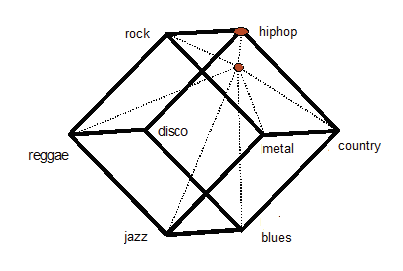
\includegraphics[width=0.5\textwidth]{cube}
\end{figure}

\section{Metrics}

There are two general types of data, qualitative and quantitative data. Qualitative data are data that cannot be measured by numbers while quantitative can be measured by numbers. Since this research will only make use of quantitative measurements, qualitative will no longer be discussed.

\subsection{Quantitative}

When using clustering as the method for machine learning, for example k-means clustering, there will result in k number of clusters after the algorithm is performed. Azcarraga \& Flores (2016) used k-means clustering in clustering the 1 second music segments. The best matching unit (BMU) for each 1 second music segment is first computed using Euclidean distance, which is the square root of the square of the difference between the x-axis of the first and second point added to the square of the difference between the y-axis of the first and second point, as shown in Figure 3.5.

\begin{figure}[h]
\caption{Euclidean Distance Diagram}
\centering
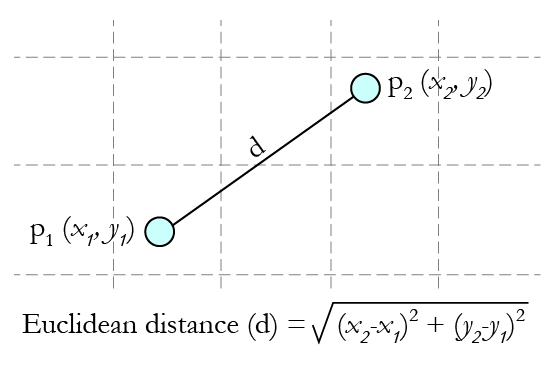
\includegraphics[width=0.5\textwidth]{euclidean}
\end{figure}

Each time a 1 second music segment has a BMU inside a cluster, the frequency count for that cluster is incremented. In this way, only the clusters that are mainly used by the music or symphony will have a high frequency count. The frequency counts are then normalized by dividing the counts of a certain composition by its total number of 1 second music segments. Once these normalized frequency counts are summarized, the resulting percentages can then be used to perform pair-wise comparisons between symphonies as shown in Appendix D.

\nocite{Dubnov}
\nocite{Azcarraga2016}
\nocite{cambouropoulosEmilios}
\nocite{3dsom}
\nocite{correa}
\nocite{imogen}
\nocite{libin}
\nocite{foote}
\nocite{silla}
\nocite{mcfee}
\nocite{hepokoski}
\nocite{heikkinen}
\nocite{bbc}
\nocite{huron}
\nocite{mckay}
\nocite{mcennis}
\nocite{loughran}
\nocite{lutter}
\nocite{mermelstein}
\nocite{agarwal}
\nocite{iitg}
\nocite{ng}
\nocite{mccria}
\nocite{brownlee}
\nocite{germano}
\nocite{bullinaria}
\nocite{kropotov}
\nocite{grabczewski}
\nocite{gupta}
\nocite{brownlee1}
\nocite{trevino}
\nocite{hartigan}
\nocite{brown}
\nocite{ziv}
\nocite{ron}
\nocite{mitchell}
\nocite{guyon}
\nocite{yang}
\nocite{kohonen}
\nocite{maaten}
\nocite{rumelhart}
\nocite{storkey}